% !TEX TS-program = pdflatex
% !TEX encoding = UTF-8 Unicode

% This is a simple template for a LaTeX document using the "article" class.
% See "book", "report", "letter" for other types of document.

\documentclass[11pt]{article} % use larger type; default would be 10pt

\usepackage[utf8]{inputenc} % set input encoding (not needed with XeLaTeX)

%%% Examples of Article customizations
% These packages are optional, depending whether you want the features they provide.
% See the LaTeX Companion or other references for full information.

%%% PAGE DIMENSIONS
\usepackage{geometry} % to change the page dimensions
\geometry{a4paper} % or letterpaper (US) or a5paper or....
% \geometry{margin=2in} % for example, change the margins to 2 inches all round
% \geometry{landscape} % set up the page for landscape
%   read geometry.pdf for detailed page layout information

\usepackage{graphicx} % support the \includegraphics command and options

% \usepackage[parfill]{parskip} % Activate to begin paragraphs with an empty line rather than an indent

%%% PACKAGES
\usepackage{booktabs} % for much better looking tables
\usepackage{array} % for better arrays (eg matrices) in maths
\usepackage{paralist} % very flexible & customisable lists (eg. enumerate/itemize, etc.)
\usepackage{verbatim} % adds environment for commenting out blocks of text & for better verbatim
\usepackage{subfig} % make it possible to include more than one captioned figure/table in a single float
\usepackage[section]{placeins} %add the command \floatbarrier at the end of each section
 \usepackage{floatrow}
% These packages are all incorporated in the memoir class to one degree or another...

%%% HEADERS & FOOTERS
\usepackage{fancyhdr} % This should be set AFTER setting up the page geometry
\pagestyle{fancy} % options: empty , plain , fancy
\renewcommand{\headrulewidth}{0pt} % customise the layout...
\lhead{}\chead{}\rhead{}
\lfoot{}\cfoot{\thepage}\rfoot{}

%%% SECTION TITLE APPEARANCE
\usepackage{sectsty}
\allsectionsfont{\sffamily\mdseries\upshape} % (See the fntguide.pdf for font help)
% (This matches ConTeXt defaults)

%%% ToC (table of contents) APPEARANCE
\usepackage[nottoc,notlof,notlot]{tocbibind} % Put the bibliography in the ToC
\usepackage[titles,subfigure]{tocloft} % Alter the style of the Table of Contents
\renewcommand{\cftsecfont}{\rmfamily\mdseries\upshape}
\renewcommand{\cftsecpagefont}{\rmfamily\mdseries\upshape} % No bold!

%%% END Article customizations
 \usepackage{fixltx2e}
\usepackage{authblk}
\usepackage[english]{babel}



%%% The "real" document content comes below...

\title{Visual Rendering \& Oculus Rift}
\author{Marco Godi \& Francesco Giuliari}
\affil{Università degli Studi di Verona}
%\date{} % Activate to display a given date or no date (if empty),
         % otherwise the current date is printed 

\begin{document}
\maketitle



\tableofcontents





%%%%%%%%%%%%%%%%%%%%%%%%%%%%%
%%%%%        Introduction        %%%%%%%%%%%%%%
\newpage
\begin{abstract}
\textbf{ This paper is the description of a software project which aims to explore new possibilities offered by the Oculus Rift headmount display. The focus is the study of Volumetric Rendering of 3D datasets (mainly medical results) in a Virtual Reality environment. The possible user base could be the medical field: there are many obvious advantages in a full immersion environment which allows the visualization of medical data in realtime. }
\end{abstract}
\section {Introduction}


%%%
\subsection{Volumetric rendering}
Volumetric rendering is the name used to describe techniques used to display a 2D projection of a 3D data set. It differs from ``normal'' rendering techniques because while being more costly (in term of hardware minimum requirements) it offers more the opportunity to interact with the 3D model so we can cross section the model, see his internal components and overall get more information at run time.  

%%%
\subsection{The Oculus Rift}
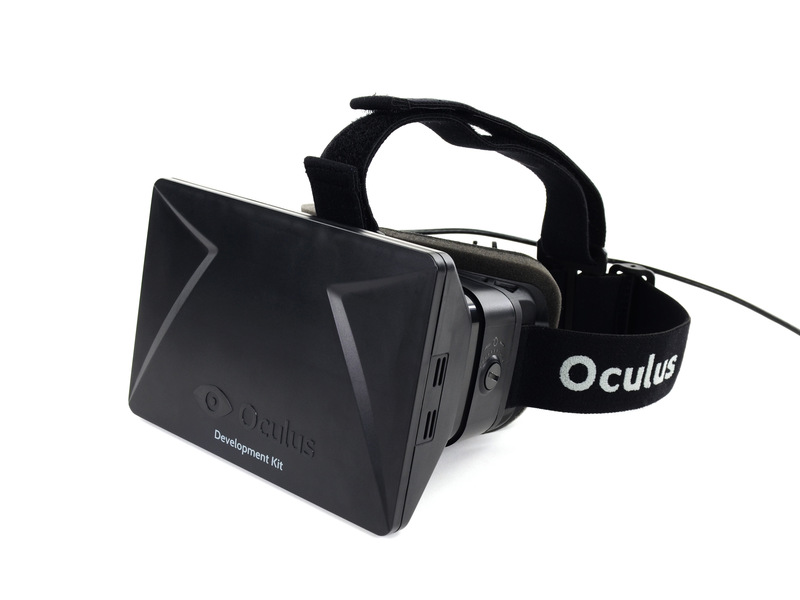
\includegraphics[scale=0.5]{oculus.jpg}

The Oculus Rift  is a virtual reality headset by Oculus VR that offer the user a fully immersive experience so they can see and interact with the application as if he was seeing with his own eyes instead of looking at a monitor. As of today the most advanced model is the DK2, for this project we're using the DK1. Our application is not compatible with DK2 because the approach we used is not supported on the newer model and the updated approach needs a more in-depth knowledge of the OpenGL pipeline. Luckily anyone with the required knowledge can further develop our application and make it compatible by modifying the code where the distortion is applied (More details on later sections).






%%%%%%%%%%%%%%%%%%%%%%%%%%
%%%       Requirements         %%%%%%%%%%%%%



\newpage
\section{Requirements}

%%%
\subsection{Hardware}
\begin{itemize}
\item It needs a fairly powerful computer (expecially a powerful video card) to run smoothly because the Volumetric rendering is a resources hungry technique and, since the oculus needs to have a different texture for both of the eyes, the rendering cost is doubled.

\item The graphic card needs to be able to use at least OpenGL 3.1 .

\item Oculus Rift DK1
\end{itemize}


%%%
\subsection{Software}
\begin{itemize}
\item The application at the moment only supports Windows operationg system since it uses OS dependant libraries, it was developed and tested on Windows 8.1.
\item To succesfully use the Oculus Rift headest the needs to have the Oculus Runtime software available at the Oculus VR official website.
\end{itemize}












%%%%%%%%%%%%%%%%%%%%%%%%%%%
%%             External Libraries               %%%%%%%%%%

\newpage
\section{External Libraries}
Since this project needed to be completeted in a fairly reasonable amount of time we decided to use some external libraries for an easier management, for the volumetric rendering we're using the VTK libraries, and, for the Oculus Rift management we're using the Oculus SDK libraries.

%%%
\subsection{VTK}
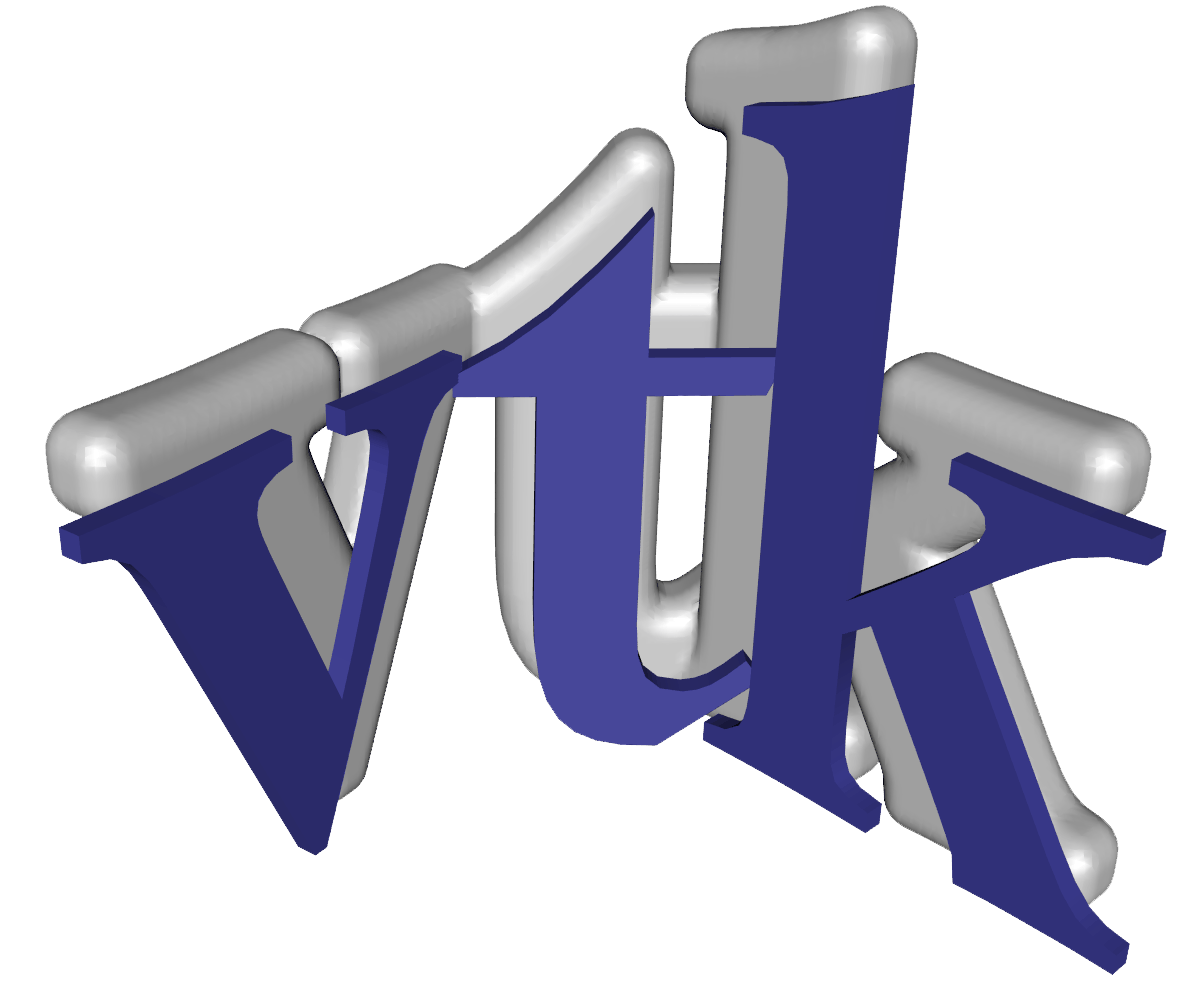
\includegraphics[width=0.2\linewidth]{VTK.png}

The Visualization Toolkit (VTK) is an open-source, freely available software system for 3D computer graphics, modeling, image processing, volume rendering, scientific visualization, and information visualization. VTK also includes ancillary support for 3D interaction widgets, two- and three-dimensional annotation, and parallel computing. At its core, VTK is implemented as a C++ toolkit, requiring users to build applications by combining various objects into an application. The system also supports automated wrapping of the C++ core into Python, Java, and Tcl, so VTK applications may also be written using these interpreted programming languages.
Using the VTK framework has many pros and cons.
Pros:
\begin{itemize}
\item We don't need to worry about creating the graphical environment, VTK takes care of creating a window and setting up OpenGL libraries for use. The advantage is that this works across different OSs, so in the future it will be relatively easy to make this software work on platforms other than Windows if this is required since VTK supports Windows, Linux and OS X.
\item VTK natively includes volumetric algorithms, so we don't need to worry about researching and implementing them. With the recent (at the time of writing) 6.2 update, updated algorithms are available (but they will be more stable in the future versions). In theory this application could have state of the art algorithms just by keeping the VTK library updated, with minimal effort on the developing side.
\item VTK also supports many commonly used 3D dataset file extensions, such as DICOM (which is standard in medical data).
\end{itemize}
Cons:
\begin{itemize}
\item VTK has its own pipeline. This means that to develop with VTK you have to follow the library own way of developing the application. A big problem during development was figuring out where to use Oculus SDK since it requires intervention on the rendering cycle, which is normally hidden to the programmer in a VTK application.
\item VTK has some annoying shortcomings in many things. An example of this is setting up fullscreen, which required a nasty hack to overcome. Luckily this particular bug was corrected with version 6.2
\item An extensive documentation is available (complete with examples) . While this is a good thing (not counting some of the mistakes or shortcomings) it also is a problem because of the sheer number of classes which are part of the library. Sometimes is very difficult finding which class you need to do a particular thing only (sometimes a relevant example is available).
\end{itemize}

%%%%
\subsection{Oculus SDK}
\includegraphics[width=0.4\linewidth,clip,trim=7cm -3mm 5cm -2mm]{Oculus_sdk.png}

The Oculus SDK is the libraries offered by Oculus VR to manage Oculus Rift headset implementation. It offer methods to keep tracking of the headpose, obtain hardware specifics form the Oculus headset and it allow for creation of virtual heaset useful for debugging the application.
Using OculusSDK is the recommended (and probably the only) way to interface the software with the Oculus Rift.










%%%%%%%%%%%%%%%%%%%%%%%%%%%%
%%%%%%%    Project     %%%%%%%%%%%%%%%%



\newpage
\section{Project}

%%%
\subsection{Approach}
The application uses the VTK libraries to load the Dicom files (or MHA or VTI files) which are to be visualized as a 3D dataset by a volumetric algorithm, then creates a split screen which shows two different points of view of the visualized dataset (representing the two eyes of the user) with the appropriate distance determined by the eye spacing and then applies a barrel distortion shader so that the image is fixed to display properly on the Oculus Rift.

%%%
\subsection{Classes}

%
\subsubsection{Main}
This class has the main function which is obviously the entry point for the program. The command line options are passed at the SmartVolume class, then a custom rendering pipeline is set up to allow postprocessing (in the vtkStereoDistortPass) for the split vision and the barrel distortion, then we use a utility class defined here to enable Oculus headpose tracking before finally starting the application.

\begin{figure}[h!]
  \centering
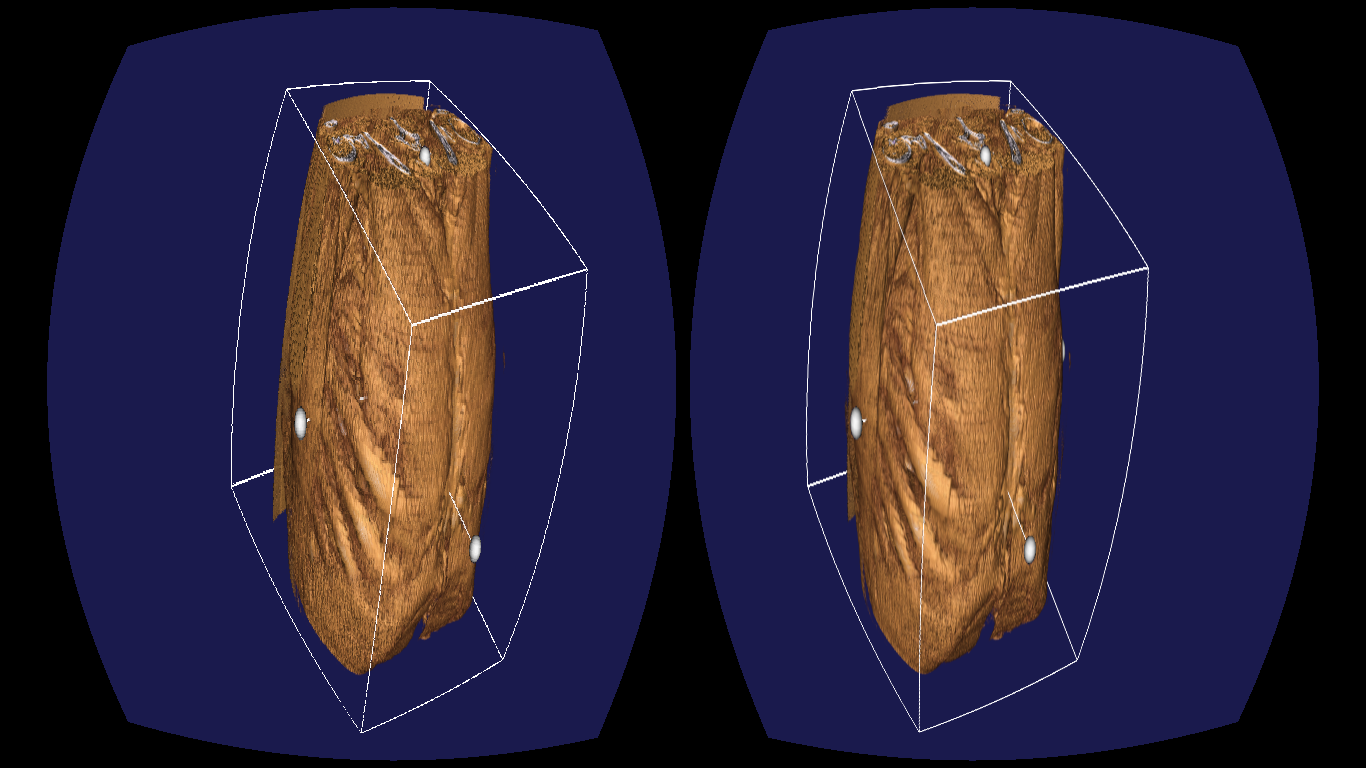
\includegraphics[width=1.0\linewidth]{img/main_using.PNG}
  \caption{The end result of the output as seen on a normal screen.}
  \label{endResult}
\end{figure}

%
\FloatBarrier
\pagebreak
\subsubsection{SmartVolume}
This class can receive command line options (you can pass them through the Init method) which are described in the PrintUsage function. The purpose of this class is to create the graphical environment(window with model and interactions), to load the requested input data (which MUST be passed through string arguments, if DEBUG is enabled it opens the "abdomen" DICOM dataset in the project folder), to visualize it with the requested blending mode (which are the different ways to map the dataset density values to the desired RGBA data) and to offer interaction with it through mouse and keyboard.

\begin{figure}[h!]
  \centering
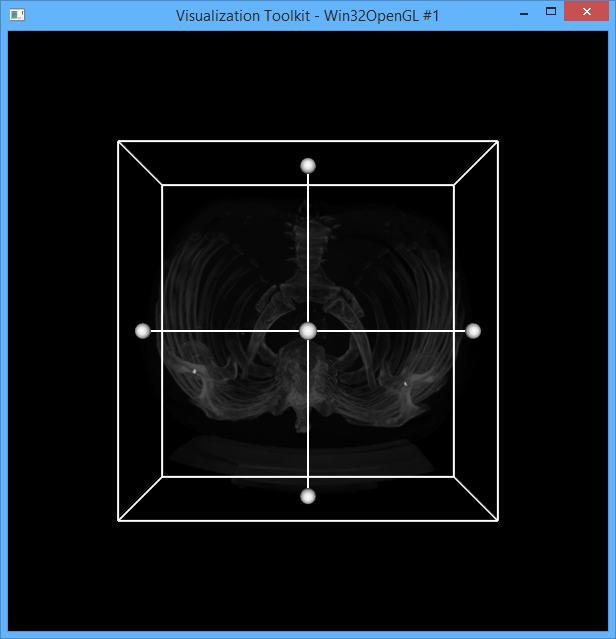
\includegraphics[width=0.4\linewidth]{img/smartvolumetricdemo_startscreen.PNG}
  \caption{Output of the SmartVolume class.}
\end{figure}

With the mouse you can rotate the model and interact with an optional bounding box around the model which allows you to cross section the dataset on your desired plane.
With the keyboard you can change the blending mode, reset the model position, change the opacity levels.

\begin{figure}[h!]

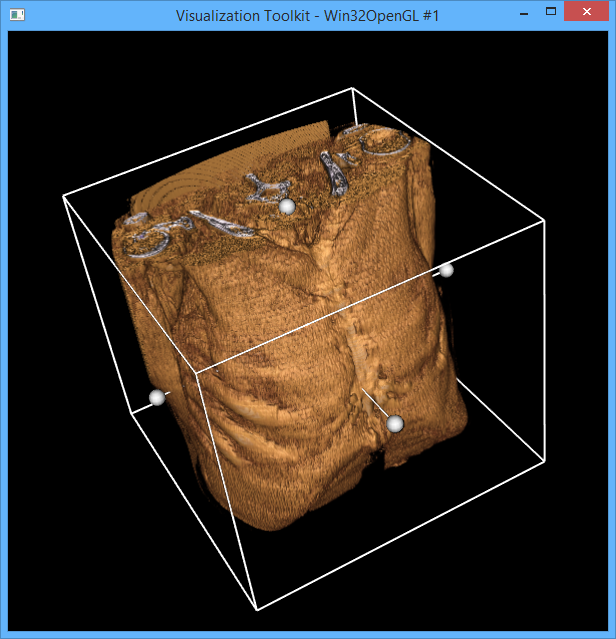
\includegraphics[width=0.4\linewidth]{img/smartvolumetricdemo_blending.PNG}
  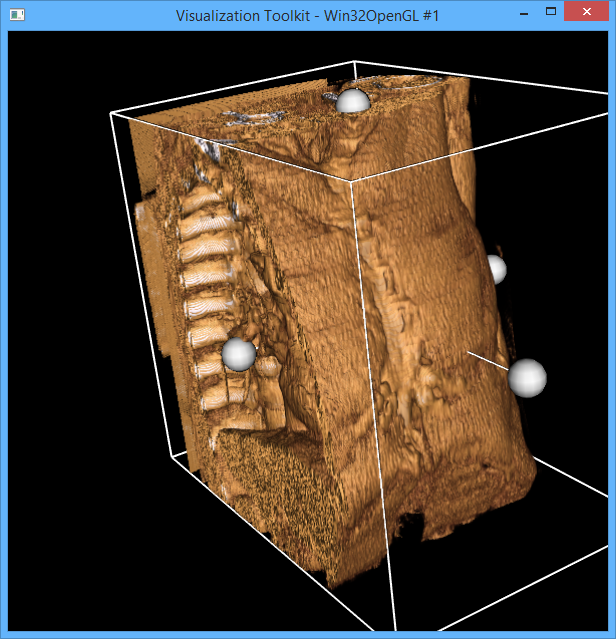
\includegraphics[width=0.4\linewidth]{img/smartvolumetricdemo_crosssection.PNG}
  \caption{The model can be rotated and also sliced.}


\end{figure}

The key bindings are in the KeypressCallbackFunction function, while the mouse interaction is defined in the VTK default  vtkInteractor.

Some local variables of significance:
\begin{itemize}
\item opacityWindow e opacityLevel together represent the range of values of density in the dataset in which the alpha value is set (from 0 to 1 from start to end in the range).
\item reductionFactor goes from 0.0 to 1.0 and represents the percentage of samples taken from the dataset (reducing this value increases performance at the cost of quality.
\item initCam and boxtrans are used in the reset function bound the the R key.
\end{itemize}

%
\FloatBarrier
\pagebreak
\subsubsection{VtkStereoDistortPass}
This class intervenes at every rendering cycle. At a conceptual level, it renders the scene two times from two slightly translated positions, and then puts them together after barrel distorting them.
This is the scene rendered two times
\begin{figure}[h!]

%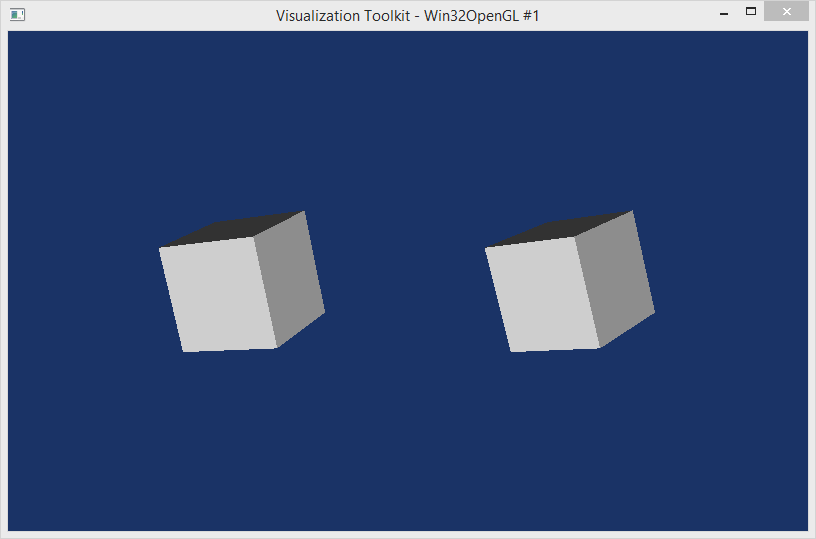
\includegraphics[width=0.8\linewidth]{img/stereodistortpass_stereoonly.PNG}
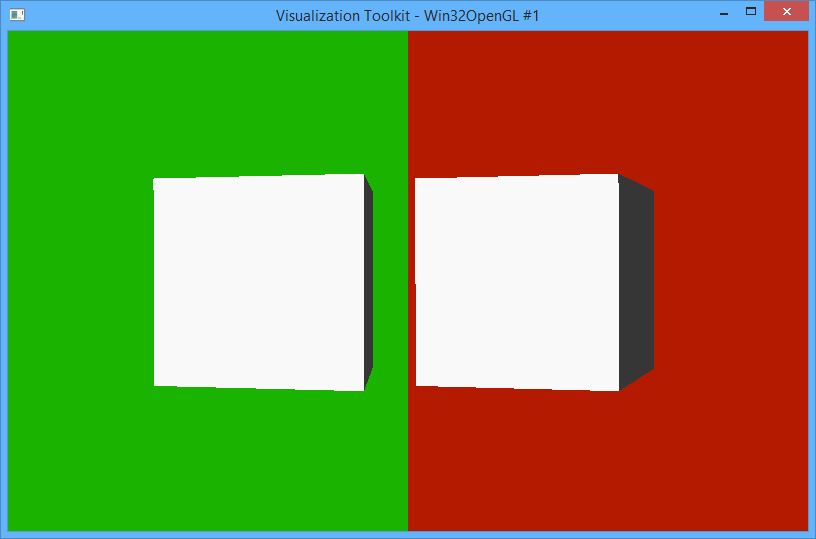
\includegraphics[width=0.8\linewidth]{img/stereodistortpass_eyedistance.PNG}
  \caption{You can see here the translated eye position.}

\end{figure}


This is realized by using a fragment shader with two textures as input. It needs a value for the InterPupillaryDistance to be set. A lot of code is just setup for the Textures, the FBOs and the ShaderProgram.


The fragment shader (distortion.fs) determines whether the pixel is in the left or the right part of the screen and calculates distortion coordinates accordingly (using parameters set in the vtkStereoDistortPass Class. Then it takes the corresponding pixel color from the determined texture in which the two rendered scenes are stored.
Almost all of the OpenGL and graphical setup code is based on the VTK vtkGaussianBlurPass source code.

%

\FloatBarrier

\subsubsection{Oculus\_Middleware}
This class is used as a class used to initializate the Oculus and return hardware related information such as the head pose and textures size.

\begin{figure}[h!]
	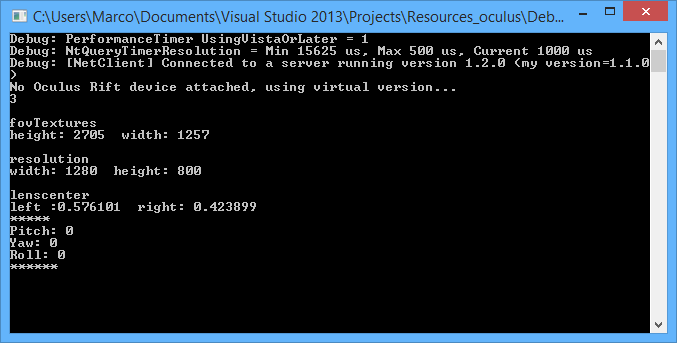
\includegraphics[width=1.0\linewidth]{img/rift_middleware.PNG}
  	\caption{Informations returned from the oculus\_middleware.}
\end{figure}





%%%%%%%%%%%%%%%%%%%%%%%%%%%%%%
%%%%%%%  Development Journal     %%%%%%%%%%%%
\newpage

\section{Development journal}
Over the course of this stage we had to go through many stages in which we were faced with different problems each one with many alternative solution. In this section will be posted which of these solutions were implemented in the project and the reasons for its choosing. 

%%%
\subsection{Volumetric rendering libraries}
The first thing we had to decide was how to handle the volumetric rendering, the possible libraries are linked below

\begin{description}

\item[Voreen]\hfill \\ 
 Voreen is an open source rapid application development framework for the interactive visualization and analysis of multi-modal volumetric data sets. It provides GPU-based volume rendering and data analysis techniques and offers high flexibility when developing new analysis workflows in collaboration with domain experts. The Voreen framework consists of a multi-platform C++ library, which can be easily integrated into existing applications, and a Qt-based stand-alone application.
 \item[VTK] \hfill \\
The Visualization Toolkit (VTK) is an open-source, freely available software system for 3D computer graphics, modeling, image processing, volume rendering, scientific visualization, and information visualization. VTK also includes ancillary support for 3D interaction widgets, two- and three-dimensional annotation, and parallel computing. At its core, VTK is implemented as a C++ toolkit, requiring users to build applications by combining various objects into an application. 
 \item[Open Inventor] \hfill \\
Open Inventor® is an object-oriented, cross-platform 3D graphics toolkit for the development of industrial-strength, interactive applications using C++, .NET or Java.
Its easy-to-use API, its extensible architecture, and its large set of advanced components provide developers with a high-level platform for rapid prototyping and development of 3D graphics applications.

\end{description}

\noindent
After a long discussion among ourselves where we studied the pros and cons of each library we decided to use the VTK libraries mainly for these two reason :
\begin{itemize}
\item Voreen, while offering a whole framework and many already implemented function, has almost no documentation and we didn't have enough time to learn it from scratch. %questa frase non mi convince, todo cambiarla
\item Open inventor is not open sourced. 
\end{itemize}

%%%
\subsection{Omegalib}
Now that we decided to use the VTK as volumetric rendering library, we looked up projects similar to this one so we could use that as a base or as an inspiration.After a little search we found a project that seems to be the silver bullet for our problem, that being Omegalib by UIC Electronic Visualization Laboratory.
\newline
\newline
The main features that leaded us to try using Omegalib are:
\begin{itemize}
\item It implements two rendering libraries, OpenSceneGraph and VTK.
\item It natively redirects  the output on various devices, among them is the OculusRift.
\item Support for a wide range of input peripherals (controllers, motion  capture systems, touch surfaces, speech and brain interfaces), through  the  Omicron toolkit.
\item It offers a python wrapper so that the program could be written using a simpler language.
\end{itemize}

\noindent
We decided that learning to use the Omegalib was our best bet to make this project easier to extend for future development, so we rewrote our vtk application as a python script.

On paper the last thing that needed to be done was assigning the oculus rift configuration to the application, but when we tried doing that it didn't work and the results weren't as expected.

We attempted  reviewing the whole library code that manage the output control, specifically how it interacted with the oculus rift configuration and then contacted the Omegalib developer on the project mailinglist to see if there was a way to see what the problem was and how to resolve it.
Turns out that, while Omegalib implements the VTK, it doesn't support the volumetric rendering, at least it doesn't as of now, it may be implemented in the future.

Because of this any and all plans of using Omegalib for this project fell through so we were back at the beginning and had to go with pure VTK again.

\subsection{Pure VTK approach}

So what we needed was to find a way to implement all of these features:
\begin{itemize}
\item Volumetric Visualization of 3D datasets
\item "Two points of view" management (for the two eyes of the Oculus user)
\item Applying barrel distortion
\item Inserting head pose tracking into a VTK application
\item Outputting video on the Oculus Rift
\end{itemize}

%link qui o li mettiamo in fondo nelle citazioni? MI DA ERRORE QUA NON SO COSA
We looked for other similar projects and two caught our attention: multipass\_vtk by zadacka ( https://github.com/zadacka/multipass\_vtk ) and and application by  Przemysław Brudny and Mateusz Wójcik by the Universidade de Aveiro ( which you can find here http://sweet.ua.pt/paulo.dias/rva/TrabalhosRVA\_2.htm ).

The first one sadly only supports Linux and uses an older version of  the Oculus SDK, but uses an interesting approach (the multipass system offered by VTK) which we'll look more into later.

The second one uses a software distortion of the image, making it far too slow for an interactive experience and, like the first one, it also uses an older version of the Oculus SDK

While we were studying these projects, we started developing other components of our software.
Starting from a VTK example, we created a Volumetric viewer which takes a series of .dcm files (or a .vti or a .mha) and visualizes it on screen, making it possibile to manipulate it by moving the camera and using widgets to make cross sections of it in real time.
%screen del Volumetric Viewer

While we were looking into a way to apply a barrel distortion and output our software onto the Oculus Rift, we also created a program which visualized onto two viewports on a split screen a normal VTK application, each viewport having a translated camera based on the eye distance value. We made this software and it worked, but then we discarded it because we found another solution, easier to manage and less verbose.

We also looked into pre-existing OpenGL Oculus Rift applications to get an idea about how to make a VR software. We found very soon that the latest way to do it involved pure OpenGL which is very problematic to use in a VTK application without knowing it very well because you could mess withthe VTK pipeline. So we opted for a deprecated way, which includes distortion using a shader in post-processing and using Mirrored Desktop so you can use the Oculus as an external monitor.

So we learned of two ways to apply post processing into a VTK application:
\begin{itemize}
\item The external way: WindowToImageFilter, which ``takes a screenshot" of a viewport and lets you use it as an Actor2D... Two problems: it's very slow (it loads the screenshot from video memory to RAM and the to video memory again) and also doesn't support shaders.
\item The internal way: Multipass ( inspired by zadacka's multipass\_vtk ) which lets you build the rendering pipeline of an application, sometimes down to the OpenGL code. Using a Gaussian Blur Post Processing example as a starting point we built a class which solves two of our needed features: "Two points of view" (by making the render pass render the scene two times from different positions) and barrel distortion (by applying a shader to the texture in which we store the rendered scene).
\end{itemize}
So we had a volumetric viewer, we could have video from our two eyes, we could distort it and output all of this into our Oculus Rift by mirroring the screen.
We only needed to handle the user's Head Pose, which we did by polling it trough the Oculus SDK every few milliseconds.

%Putting it all together we realized our software.

For an easier use of the software we also created a simple Java application that functions as a launcher for our software, allowing to choose in an interactive way the dataset to be visualised, without forcing the use of a command line.

\subsection{Future expansion}
At the current time, we have a working prototype of the application. It was tested with different datasets in different file formats. It still needs some tweaking on the distortion, but the minimal goals we set at the beginning of the development are met.

But the project is far from completed, in fact there are many new features that could be added. Here are some examples, complete with suggestions of how you should look into doing it.
\begin{itemize}
\item \textbf{Hand Tracking and Gesture Recognition support} could be a useful feature. The obvius advantage would be having an intuitive way to interact with the software, allowing an easy access even to not computer-savyy people which could be found, for example, in the medical field (which is the main userbase we focused on). In theory the integration with our application should not present particular problems. The recommended way to implement it would be similar to the Oculus Rift HeadPose polling (a repeating timer which polls the Gesture Recognition hardware and makes the application respond to the user gestures). Recommended hardware are Kinect by Microsoft and Leap Motion.
\item \textbf{DK2 Support} is a very important feature to develop. Right now the software works only with DK1 because of the distortion and output method we chose to use. Our reasons to do that is that it was the easier one to implement and the only one we were able to do in a reasonable time. Right now we used the "Client Distortion Rendering" (refer to the Oculus Developer Guide on the Oculus Website for details) and we used a deprecated way of rendering to the Oculus because it was within our abilities (using Windows 8 Duplicate monitor option)
\item \textbf{Miscellaneous features} such as user personalization of the volumetric transfer function, or a more user friendly interface, or the possibility to switch between rendering in a window or on the Oculus  at run-time
\end{itemize}
\newpage

\section{Conclusions}
Now that we worked with both of the two main features of this software (Volume Rendering and Virtual Reality) we can make a few observations.

\begin{itemize}
\item We noticed that the combination of these two features is very resource-hungry. Volumetric Rendering can make rendering very slow, even with state of the art algorithms. The situation is even worse with virtual reality since you need double the time for every rendering cycle  (two slightly different volume renders of the same dataset) and it also has to be rendered with a framerate equal to the device refresh rate or the end result will be sloppy and could cause motion sickness. This problem can be mitigated in this software by using the command line argument "reductionFactor", which is a value between 0.0 and 1.0 that determines the ratio of the points of the dataset to be shown. This allows for an increase of rendering speed at the cost of quality.

\item During testings of the software we noticed that, while we can give the user an immersive experience,
the advantage of doing this is not much. Virtual reality is a wonderful tool in fields like 
gaming and simulators on the other hand it is not as usefull in other applications.

For example, immersion is not very useful when viewing medical results!
The only ``point of interest" on the scene is the model of the medical result, so there's nothing else to 
look at if you move your head, apart from a background color. Furthermore as Virtual Reality is a newly established 
technology it still has to grow before its output quality can compete against full-hd screens, 
for this reason some user may prefer a visually enhanced experience instead of an immersive one.

That doesn't mean  that this software is useless. With further development of both our software and the Oculus Rift hardware, output quality will improve. Also with the integration of Gesture Recognition and adding Position Tracking (which needs DK2 support) could make it a completely different experience.

Excluding for a moment Oculus Rift support, our application as a Volumetric Viewer per se could be useful, expecially with the addition of more features could give it the added value that would make it a useful application.

%altre conclusioni?
\end{itemize}

\newpage

\section{Bibliography}
...sort of. Since this paper is more of a development journal and software documentation, we did not see the need for quotes for other works.

Nonetheless our work was based on pre-existing works and documentations, which are here reported:
\begin{itemize}
\item Oculus Rift Documentation, available on https://developer.oculus.com/documentation/ . We studied these documents to learn how to integrate Oculus Rift in graphical application. Not included are the countless forum posts and blog entries we stumbled upon.
\item VTK 6.1 Documentation, available on http://www.vtk.org/doc/release/6.1/html/index.html . We used this as reference for which classes to use to reach our goals.
\item VTK C++ examples, available on http://www.vtk.org/Wiki/VTK/Examples/Cxx . We learned how to use VTK studying these examples.
\item zadacka's ``multipass\_vtk", available on https://github.com/zadacka/multipass\_vtk . We took inspiration to this work for some of the  implementaton of our software.
\item ``Application to allow the use of Oculus Rift with VTK" by Universidade de Aveiro, available on http://sweet.ua.pt/paulo.dias/rva/TrabalhosRVA\_2.htm by contacting professor Paulo Dias. We were also inspired by this work in our development
\end{itemize}

\newpage


\section{Thanks}
\addtocontents{toc}{\protect\enlargethispage{\baselineskip}}
We wish to express our thanks to Professor Andrea Giachetti for the idea of this project and his help during development.
We are also grateful to GitHub user zadacka and to Przemysław Brudny and Mateusz Wójcik by the Universidade de Aveiro for providing their examples for applications similar to our own.
We also thank Alessandro Febretti (main developer of Omegalib) because, even if we ended up discarding his library, was always answering our questions on the omegalib Google Group.
















\end{document}
